\documentclass[12pt,a4paper,english,twoside]{book}
\usepackage[german,english]{babel}
\usepackage[T1]{fontenc} 
\usepackage[latin1]{inputenc}
\usepackage{amsfonts}
\usepackage{amsmath}
\usepackage{latexsym}
\usepackage{amssymb}
\usepackage{epsfig}
\usepackage{moreverb}
\usepackage{rotating}
\usepackage{enumerate}
\usepackage{graphics, graphicx,wrapfig}
\usepackage{fancybox}
\usepackage{picinpar,varioref,floatflt}
\usepackage{ae}
\usepackage{longtable}
\usepackage{textcomp}
\usepackage{float}
\usepackage{url}
\usepackage{unizhdt}
\usepackage{caption}
\usepackage{bm}

%%%%%%%%%%%%%%%%%%%%%%%%%%%%%%%%%%%%%%%%%%%%%%%%%%

% Define the language of the diploma thesis
\selectlanguage{english}
%\selectlanguage{german}

\pagestyle{headings}

\begin{document}

%%%%%%%%%%%%%%%%%%%%%%%%%%%%%%%%%%%%%%%%%%%%%%%%%%

% Define the author printed on the cover page
\author{Simon Bachmann}
% Define the city and country of the author
\authorcity{Zurich, Switzerland}
% Define the student ID (Matrikelnummer)
\studentid{14-709-893}
% Define the title with optional subtitle
\title{Analysis of the Tangle in the IoT Domain}
% Define the supervisors
\supervisors{Sina Rafati}
% Define the submission date
\submissiondate{\today}

%%%%%%%%%%%%%%%%%%%%%%%%%%%%%%%%%%%%%%%%%%%%%%%%%%

% Make the title page
\maketitle

% Make the imprint on the back of the cover page
\makeimprint

\pagenumbering{roman}

% Include the files of the diploma thesis
%\cleardoublepage
\chapter*{Abstract}
\addcontentsline{toc}{chapter}{Abstract}

\selectlanguage{german}

Das ist die Kurzfassung...



\selectlanguage{english}

%\cleardoublepage

\tableofcontents

\cleardoublepage
\pagenumbering{arabic}
\chapter{Introduction}

\section{Motivation}
One of the biggest hurdles in distributed ledger technology (DLT) is the scalability issue. Bitcoin handles around 7 transactions per second (TPS), Ethereum 15 TPS \cite{ethereum-scale}, Litecoin 56 TPS and Ripple 1500 TPS \cite{bitcoin-tps}. Higher transaction throughput is achieved with larger block size. This is not a sustainable approach since the data that is stored in every node of the network grows linearly to the networks block size and effectively forcing people to leave the network with less storage and bandwidth capacity. 

In order to compete with Visa's 1600 TPS \cite{visa-tps}, increasing the block size is not enough. The lightning network is one proposal to solve the scalability issue by creating off chain transactions. However, it is not flawless because the funds are locked in payment channels and the transactions to open and close such payment channels are still slow and expensive. Ethereum is working on a solution that works similar to database sharding, where every node is storing only a portion of all the transactions on the network. However, this requires additional mechanisms such that nodes must not trust other shards in order to verify transactions that are stored in other shards.

All the DLTs mentioned previously use a linked list as a core data structure. However, a DLT created by the IOTA foundation uses a directed acyclic graph (DAG) called Tangle. This fundamental difference brings several advantages compared to traditional DLTs. However, there are other hurdles to overcome using a DAG architecture. The arguments for and against a DAG architechture in a DLT is evaluated as part of this Master Basis Module (MBM). 

\section{Description of Work}
This MBM will be conducted as a research assignment along with a 30 minutes presentation. The following topics are to be analyzed, evaluated and discussed.
\begin{itemize}
    \item A detailed analysis of the strengths and weaknesses of the Tangle's architecture and how it reaches its consensus. This also includes the problem of the coordinator and the path to full decentralization. It includes a discussion about how suitable the IOTA network is for a future project with Internet-of-Things (IoT) devices.
    \item Analysis of possible attack scenarios including the double-spend attack, large weight attack and the parasite chain attack.
    \item Case studies in the mobility and smart energy industries.
    \item The current status, process and intentions of the Qubic project is to be analyzed which is IOTA's solution for oracle machines and smart contracts.
\end{itemize}

\section{Thesis Outline}

This thesis is structured in six Sections. Section 1 focuses on the motivation of a distributed currency that uses a directed acyclic graph (DAG) instead of a singly linked list as its core data structure. Chapter 2 familiarizes the reader with the current implementation of the Tangle. Section 3 concentrates on some of the attack scenarios that are unique to the underlying data structure. Section 4 is about the current research topics done by the IOTA foundation. An evaluation of the DAG architecture is conducted in Chapter 5, which is followed by Chapter 6 where a summary and conclusions are drawn.
\chapter{The Tangle}
This chapter covers the fundamental building blocks of the directed acyclic graph (DAG) architecture of IOTA called Tangle \cite{the-tangle}.

\section{Network Partition}

The tangle does not know the discrepancy of validating nodes (miners) and issuing nodes in a sense that Bitcoin does. Every node in the network can issue and validate transactions. A new transaction is  
what motivates nodes to validate and propagate transactions. Each node calculates statistics about the activity of its neighbors. If a neighbor appears to be lazy, it can be dropped. For this reason, a node in the network is incentivized to participate in the network, even at times when it does not issue transactions. 


\section{Transactions}\label{transactions}

As there are no miners in the network, transactions are being validated by other nodes that issue transactions themselves. In order to create a new transaction on the network, a node does the following steps:
\begin{enumerate}
    \item The node chooses two unconfirmed transactions (tips) according to a random walk algorithm which will be described in more detail in Section \ref{tip-selection}.
    \item The node is responsible for checking the validity of these two transactions. Conflicting transactions are ignored.
    \item A node has to perform a cryptographic puzzle in order to make the new transaction valid. Similar to the Proof of Work (PoW) mechanism in Bitcoin, this puzzle is solved with computational resources. The puzzle is defined by finding a nonce such that the hash of this number concatenated with some data from the approved transactions results in a number smaller than some predefined constant. This puzzle is necessary in order to prevent several attack scenarios which will be discussed in Chapter \ref{attacks}.
\end{enumerate}

The next section describes parameters which are necessary of the tangle. For all figures, a box resembles a transaction and the directed edge between nodes illustrates the approval of a transactions. In order to understand the approval algorithm, the following five parameters are defined for every transaction.
\begin{description}
    \item[weight] The weight of a transaction is defined by the amount of work that the issuing node has invested in to this transaction. The weight of a transaction resembles its importance. This measurement helps to prevent spamming and other attacks since no node can create an abundance of transactions with meaningful weights within a short period of time. 
    \item[cumulative weight] The cumulative weight of a transaction is calculated by the weight of the transaction itself plus the sum of all transactions that directly or indirectly approve this transaction. Figure \ref{fig:cumulative-weight} shows how the weight and the cumulative weight change after the new transaction \textit{X} is added, the smaller number denotes the weight of a node and the bold number represents cumulative weight of a transaction.\par
        \begin{minipage}{\linewidth}
            \centering
            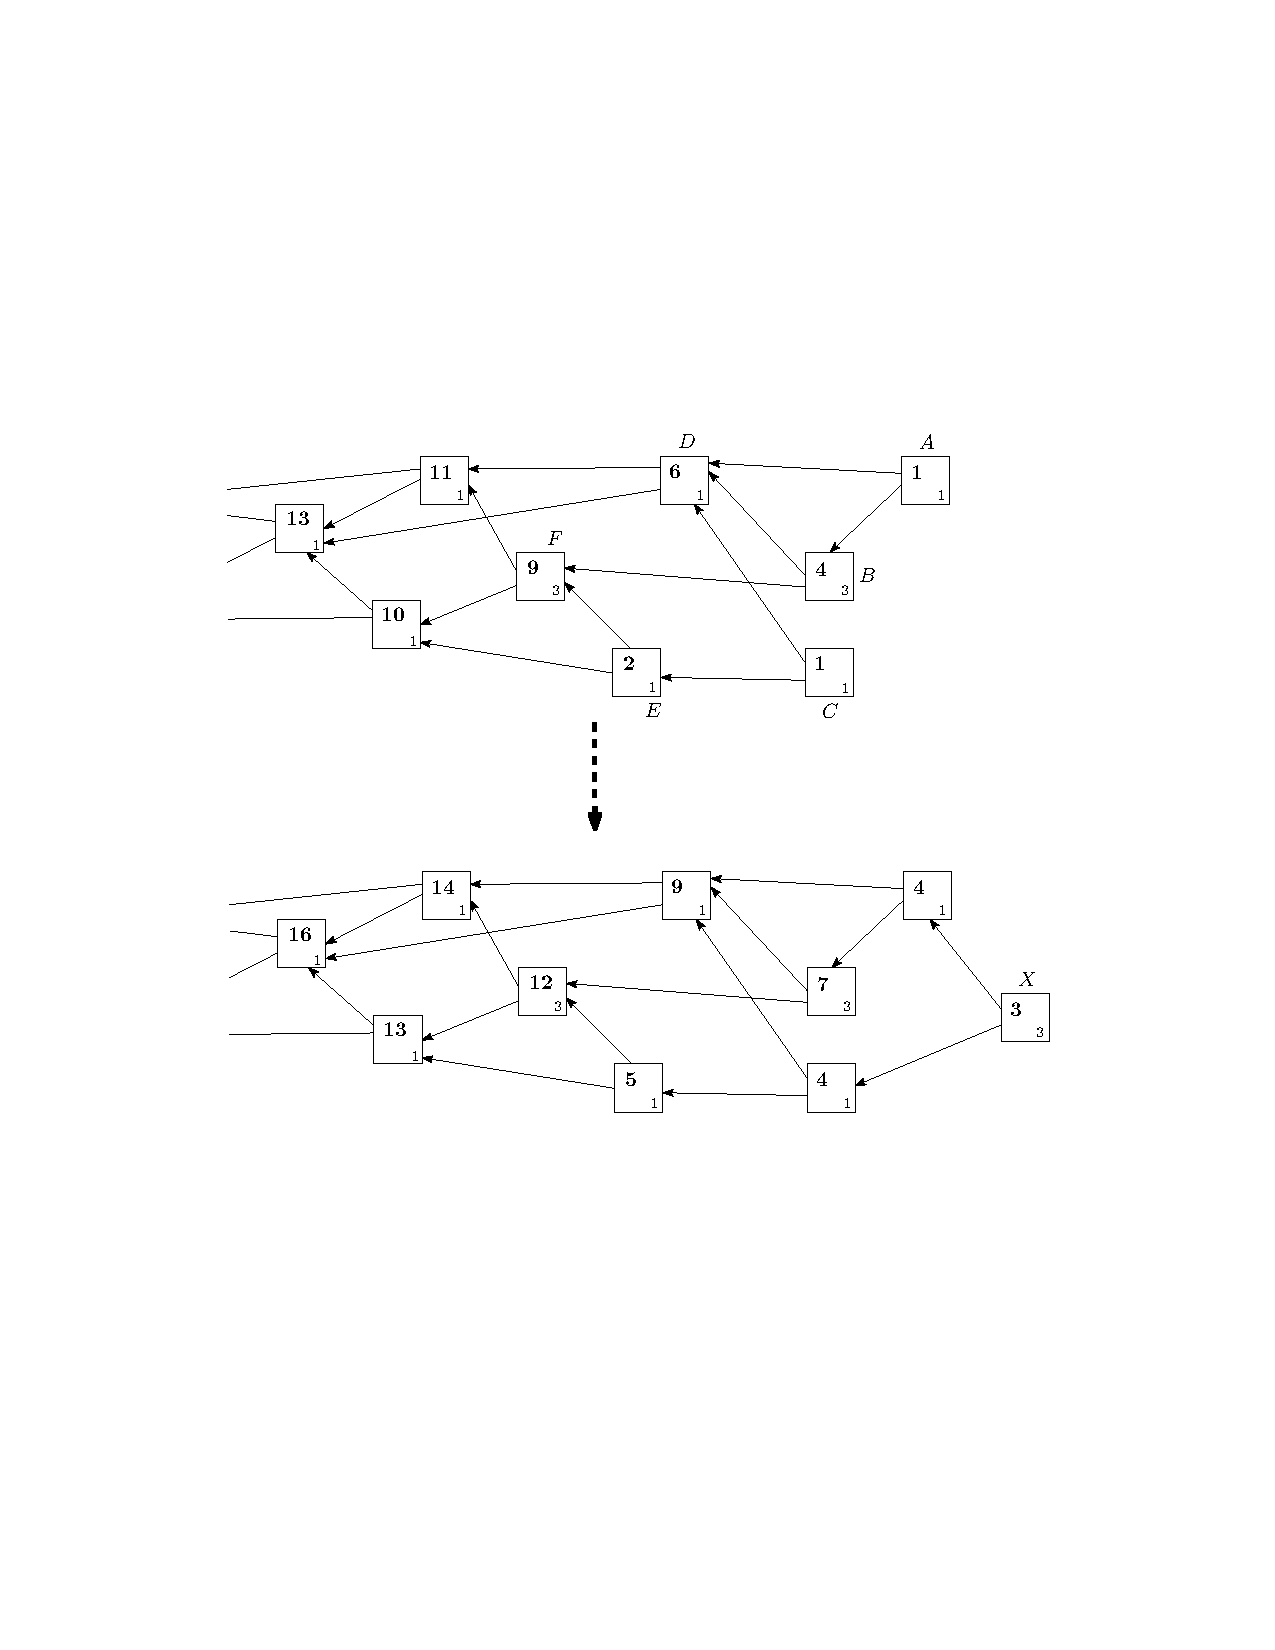
\includegraphics[width=10cm]{images/cummulative_weight.pdf}
            \captionof{figure}{Cumulative Weight \cite{the-tangle}}
            \label{fig:cumulative-weight}
        \end{minipage}
    \item[height] The height of a transaction is the length of the longest oriented path to the genesis transaction. In Figure \ref{fig:height-depth-score}, transaction \textit{G} has a height of 1 due to the blue edge.
    \item[depth] The depth of a transaction is the length of the longest reverse oriented path to some tip. In Figure \ref{fig:height-depth-score}, transaction \textit{G} has a depth of 4 due to the red approvals from newer transactions \textit{F, D, B} and \textit{A}.
    \item[score] The score of a transaction is the sum of weights of all transactions that are approved by this transaction plus its own weight. The scores for transactions \textit{A} and \textit{C} are shown with the circled number in Figure \ref{fig:height-depth-score}.\par
        \begin{minipage}{\linewidth}
            \centering
            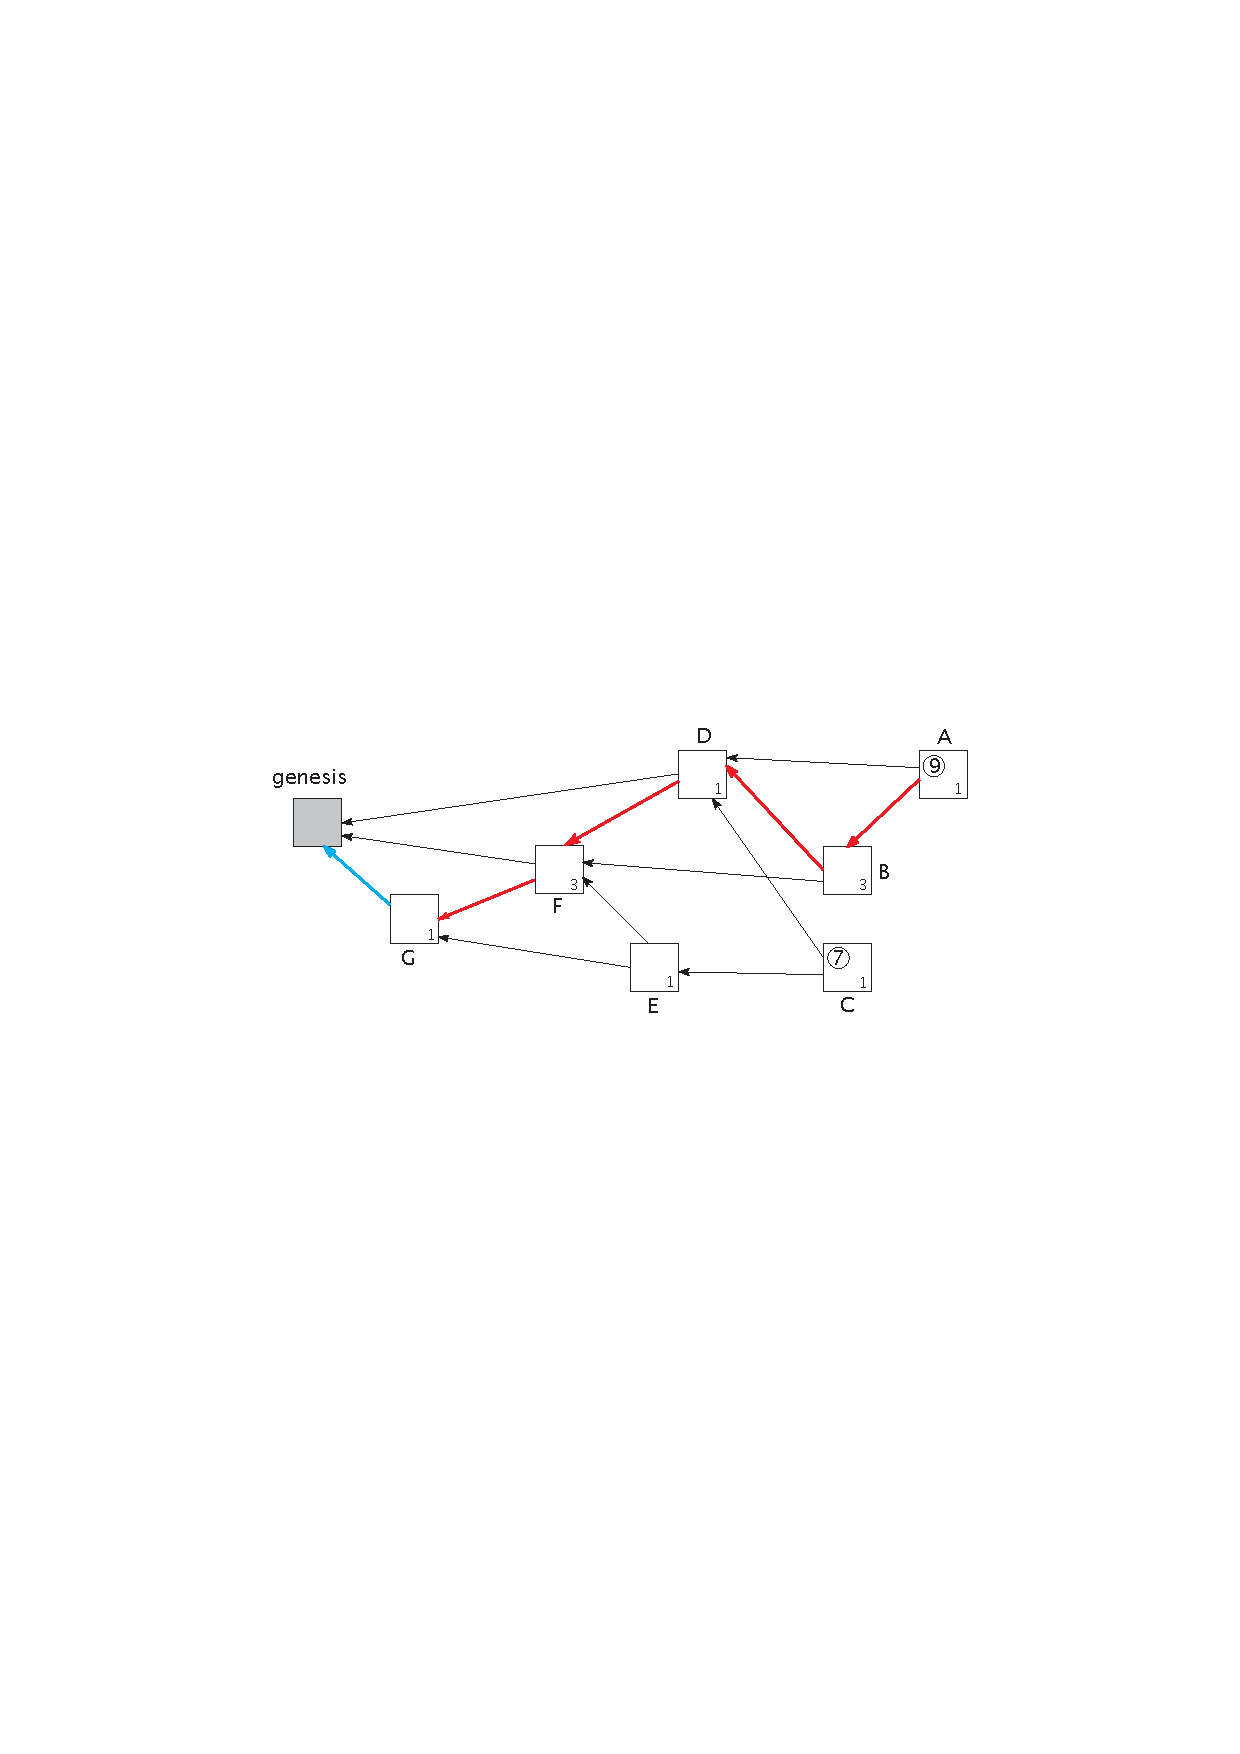
\includegraphics[width=12cm]{images/height-depth-score.pdf}
            \captionof{figure}{Height, Depth and Score \cite{the-tangle}}
            \label{fig:height-depth-score}
        \end{minipage}
\end{description}

These parameters will play an important role when discussing tip selection in Section \ref{tip-selection} and attack scenarios \ref{attacks}.

\subsection{Different Types of Transactions}\label{different-types-of-transactions}

A transaction that facilitates a transfer of IOTAs or stores data on the tangle is a bundle of transactions. Such a bundle is a combination of the following types of transactions:
\begin{description}
    \item[Output transaction] IOTA tokens are sent to another address. The value is always greater than 0 and the address is different than the address issuing the transaction bundle.
    \item[Input transaction with a positive value] These transactions facilitate a transfer to a new address in the sender's wallet.
    \item[Input transaction with a negative value] These transactions completely spend the balance of that account.
    \item[Meta transactions] These transactions have a value of 0 and make use of the \textit{signatureMessageFragment} to store data on the Tangle. 
\end{description}

Each bundle is considered as atomic. Either all or none of the transactions are accepted. Each transaction must provide its own PoW. 


IOTA represents data according to the trinary numeric system. In comparison to binary, a trinary system is more efficient in terms of computation and memory as it can represent data in three states rather than just two. Hence, a transaction is also tryte-encoded where each tryte consists of one of 27 characters.

A transaction in the IOTA protocol consists of 2673 tryte-encoded characters which are equivalent to 1.59 kBytes. Every transaction type contains the same fields. The most interesting fields are the following two.
\begin{description}
    \item[Message (2187 trytes)] This field can be used for two purposes. In case of an input or output transaction, this field contains the signature. In case of a meta transaction, these trytes can be used for storing data on the tangle. If the data is larger than 2187 trytes, the data is split among multiple transactions and grouped together in a transaction bundle. The tangle treats a transaction bundle just like a transaction. It either accepts the bundle or rejects all transactions within the bundle. The tangle explorer cannot search for a specific message. Instead, tags can be used to localize desired messages.
    \item[Tag (27 trytes)] This field is used to search for a transaction with a specific tag value.
\end{description}

Due to the design choice of quantum-resistant signature scheme, the protocol does not allow spending multiple times from the same address. Thus, a simple transaction from Alice's wallet to Bob results in the best case in a transaction bundle of three transactions. One for sending IOTA tokens to Bob, the second one for spending all the remaining IOTAs in Alice's wallet and a third one that is a meta transaction and holds the second part of the signature. Thus, the actual size of a basic Alice-to-Bob transaction results in 8019 trytes (4.77 kBytes).

\section{Tip Selection}\label{tip-selection}

Unapproved transactions are called tips. This section covers the reasons why the process of selecting a tip is important for the network.
In order to discuss the tip selection algorithm, a simulation of the DAG architecture is characterized by the following two parameters. 


\begin{description}
    \item[Transaction rate $\bm{\lambda}$] Transactions do not arrive evenly throughout time. To model such behaviour, a mathematical object called Poisson point process is used. The arrival rate of transactions is specified by the parameter $\lambda$. The higher $\lambda$ is set in the simulation, the more transactions arrive within one time-unit. If $\lambda$ is set to a really small number, the graph grows in the form of a linked list as there is always just one tip to be approved by a new transaction. Figure \ref{fig:simulation} shows a simulation, where $\lambda=5$. The tips are drawn as grey boxes.
    \item[Delay $\bm{h}$] As new transactions must perform computational work for spam prevention and this computation is based on the selected tip of that transactions, there is a delay between choosing the tips and publishing the transaction. This delay is defined by the parameter $h$. For a device with less computational power, $h$ will be larger than for computers with higher processing power. The simulation in Figure \ref{fig:simulation} assumes that $d=1$ for every device that adds a new transaction. Thus, for example the node issuing transaction 5 did not know about the transactions 1-4 when he started with the PoW computation for transaction 5. The time difference to transactions 1-4 is less than $d$. 
\end{description}

\begin{figure}[H]
    \centering
    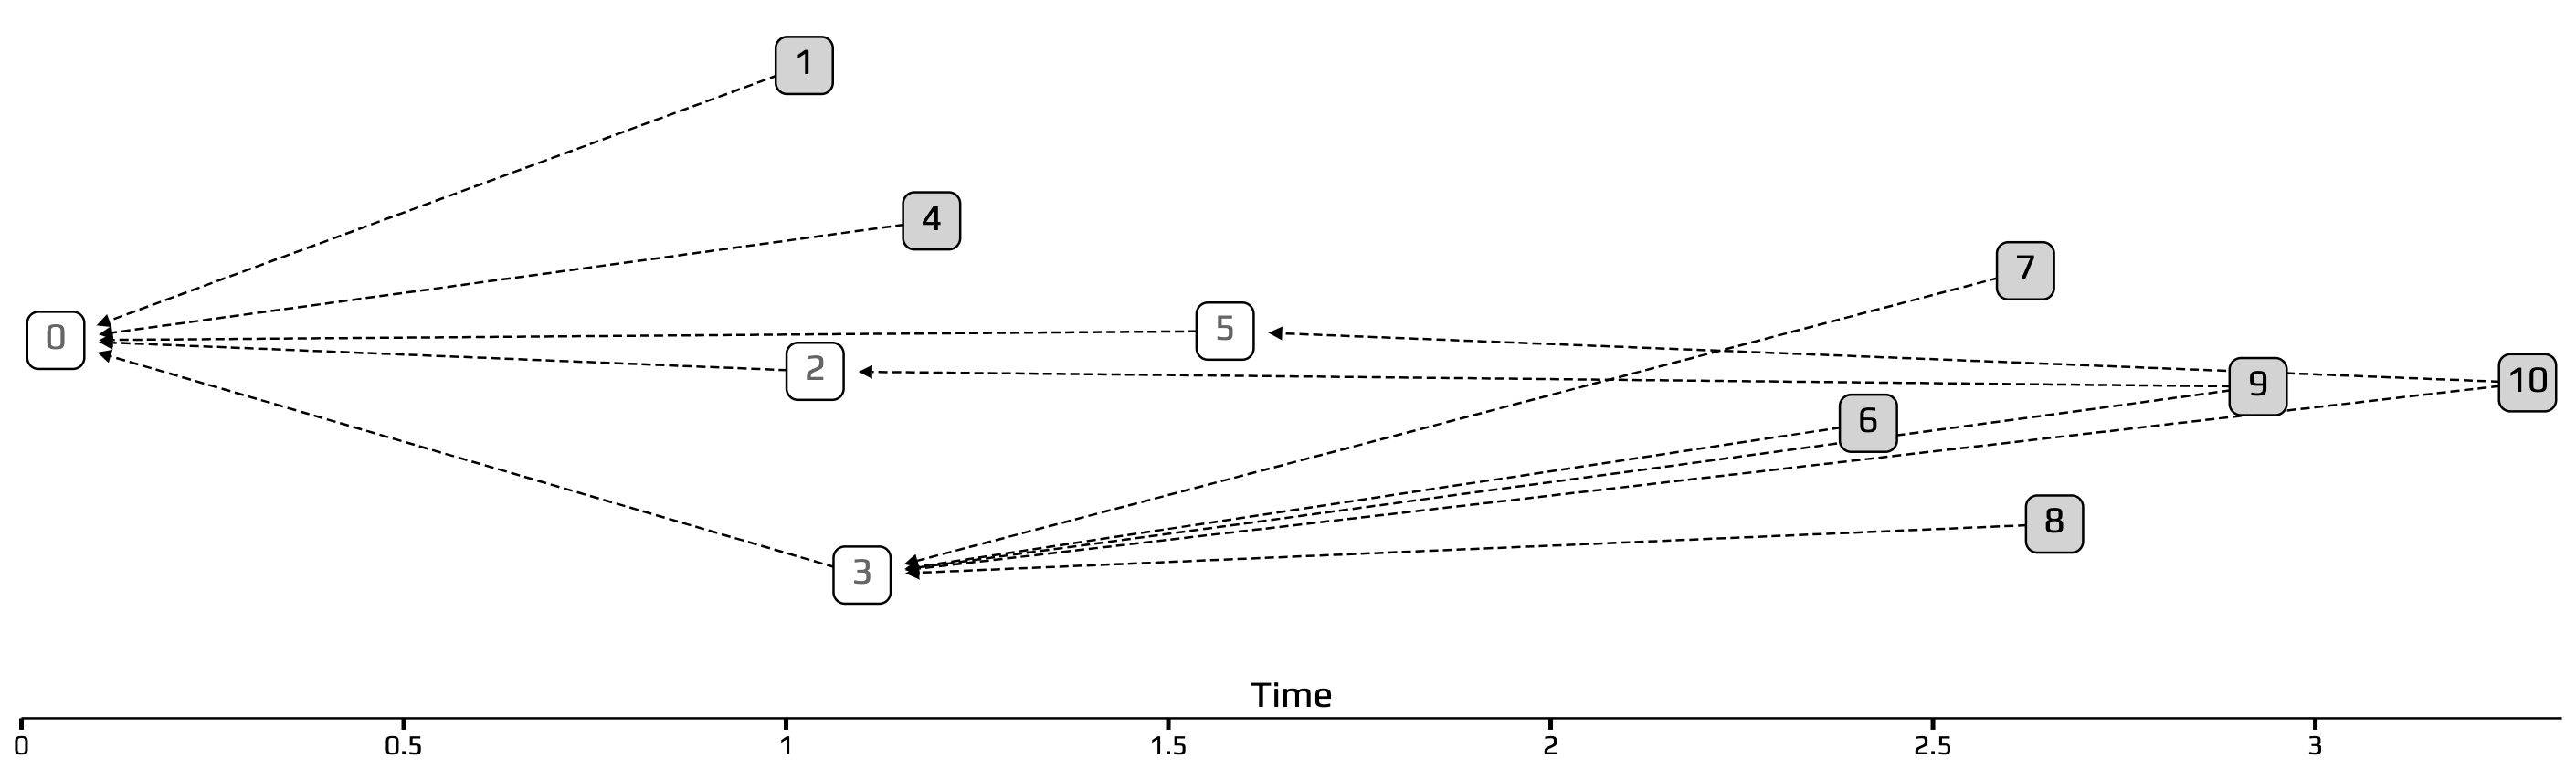
\includegraphics[width=1.0\textwidth]{images/simulation.png}
    \caption{Simulation with $\lambda=5$ and $d=1$  \cite{the-tangle-part-3}}
    \label{fig:simulation}
\end{figure}


There is a possibility that one or both of the validated transactions might no longer be a tip at the time of broadcasting the new transaction. The reason for this might be the slow computation of the required PoW or bandwidth congestion. Thus, the tangle must also accept transactions that approve already verified transactions. However, the tip selection algorithm must avoid these \textit{lazy tips} which point to older transactions. Confirming old transaction is unwanted since it increases the branching factor of the graph and thus, it increases the number of tips. Furthermore, \textit{lazy} nodes do not help the network to grow since no unapproved transactions are confirmed. In Figure \ref{fig:lazy-tip}, transaction 14 is added to the network by a lazy node. 


\begin{figure}[H]
    \centering
    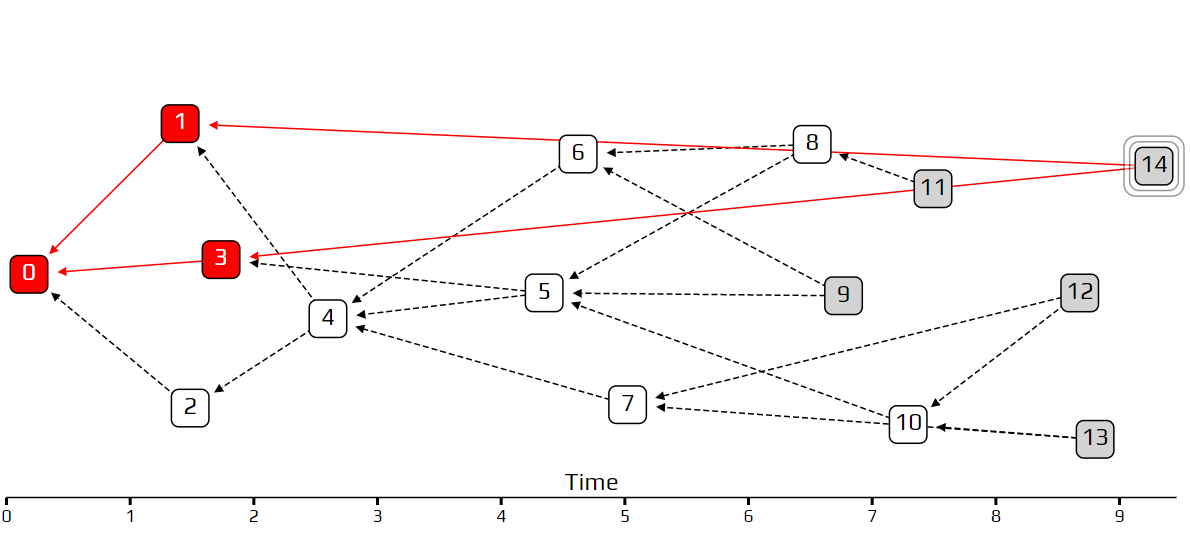
\includegraphics[width=1.0\textwidth]{images/lazy-tip.png}
    \caption{Lazy Tip \cite{the-tangle-part-3}}
    \label{fig:lazy-tip}
\end{figure}

For finding a tip, a node must walk from the genesis until it reaches an unconfirmed transaction. The node has to choose between multiple possible paths. If the node chooses the path solely based on the branching factor, transactions added by lazy nodes would be selected with the same probability as any other transaction. Thus, the random walk algorithm must be less biased towards lazy transactions. 
This is achieved by favoring transactions that have a higher cumulative weight. The bias factor is defined with the parameter $\alpha$. Setting $\alpha$ to a high value results in many unconfirmed transactions since most approvers choose the same path to the tip. These unconfirmed transactions are left behind and will never be accepted. Thus, determining an ideal value for $\alpha$ is crucial for the usability of the network and depends on the transaction arrival rate, the PoW delay of different devices in the network, network delay and the number of tips. 

The method of setting a rule on how to find a path towards a tip is called a Markov Chain Monte Carlo technique (MCMC) \cite{mcmc}. In a Markov chain, each step enforces a rule which is defined in advanced and does not depend on the previous step. In the example of the Tangle, each step is a node in the graph and the rules are the probabilities of the available paths depending on the cumulative weights.

Figure \ref{fig:mcmc} illustrates the simulation of a random walk algorithm. It is assumed that the network delay is 1 time unit. Thus, the node that issues transaction 9 does not know about transaction 7 and 8. As transaciton 6 confirms transaction 1, transaction 1 has a cumulative weight of 2. Therefore, it is more likely to choose the path with a higher cumulative weight.

\begin{figure}[H]
    \centering
    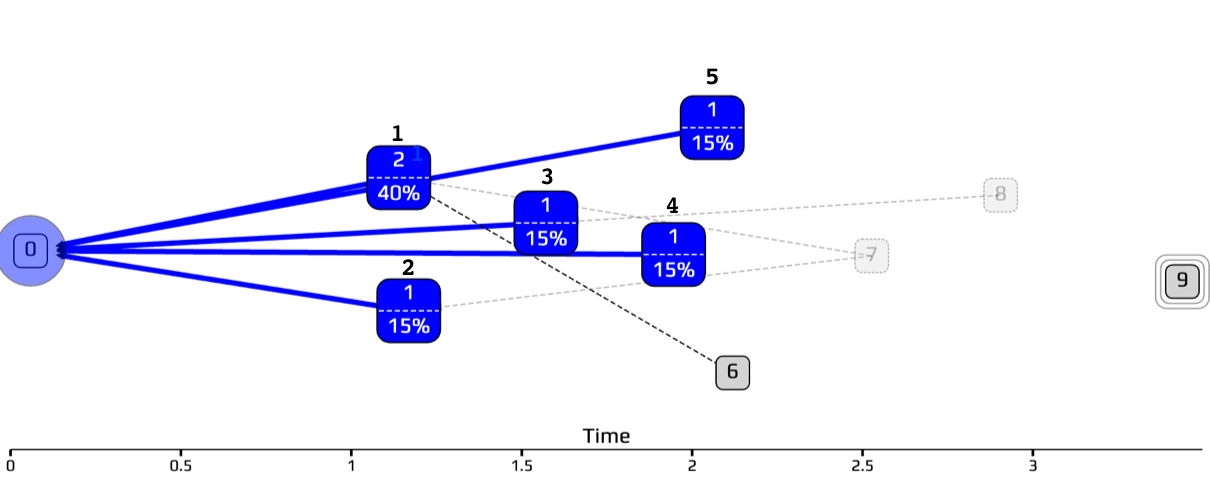
\includegraphics[width=1.0\textwidth]{images/mcmc.png}
    \caption{Markov Chain Monte Carlo Technique}
    \label{fig:mcmc}
\end{figure}

\section{Transaction Validation}\label{transaction-validation}

The transaction validation process is similar to Bitcoin's unspent transaction output (UTXO) model. An unspent transaction output is the output of a transaction that a user receives and is able to spend in the future. Thus, the validating node must check all previously made transactions of the sender address in order to verify a transaction. The smallest unit of the underlying currency is also called IOTA. All IOTA are minted in the genesis transaction and therefore, every IOTA can be traced back to genesis block. 

Transactions cannot be seen as valid as soon as one approver has referenced it. Thus, a new parameter is introduced called confirmation confidence. The confirmation confidence for a transaction $X$ can be calculated in the following way.

\begin{enumerate}
    \item The tip selection algorithm is run 100 times.
    \item The number of tips that approve transaction $X$ is counted.
    \item Every tip is weighted by the likelihood that it will be accepted in the future.
    \item The confirmation confidence of transaction $X$ is the fraction of approving transactions.
\end{enumerate}

It is assumed that transactions are issued by a large number of independent entities, so the process of incoming transactions can be modeled Poisson point process \cite{the-tangle}. $\lambda$ denotes the rate of the Poisson process and it is assumed that it remains constant in time. At some point in time, every new transaction will approve transaction $X$ since all tips include a path to transaction $X$. Thus, after the adoption period, the cumulative weight will grow linearly with $\lambda * w$ where $w$ is the average weight of a transaction.

\begin{figure}[H]
    \centering
    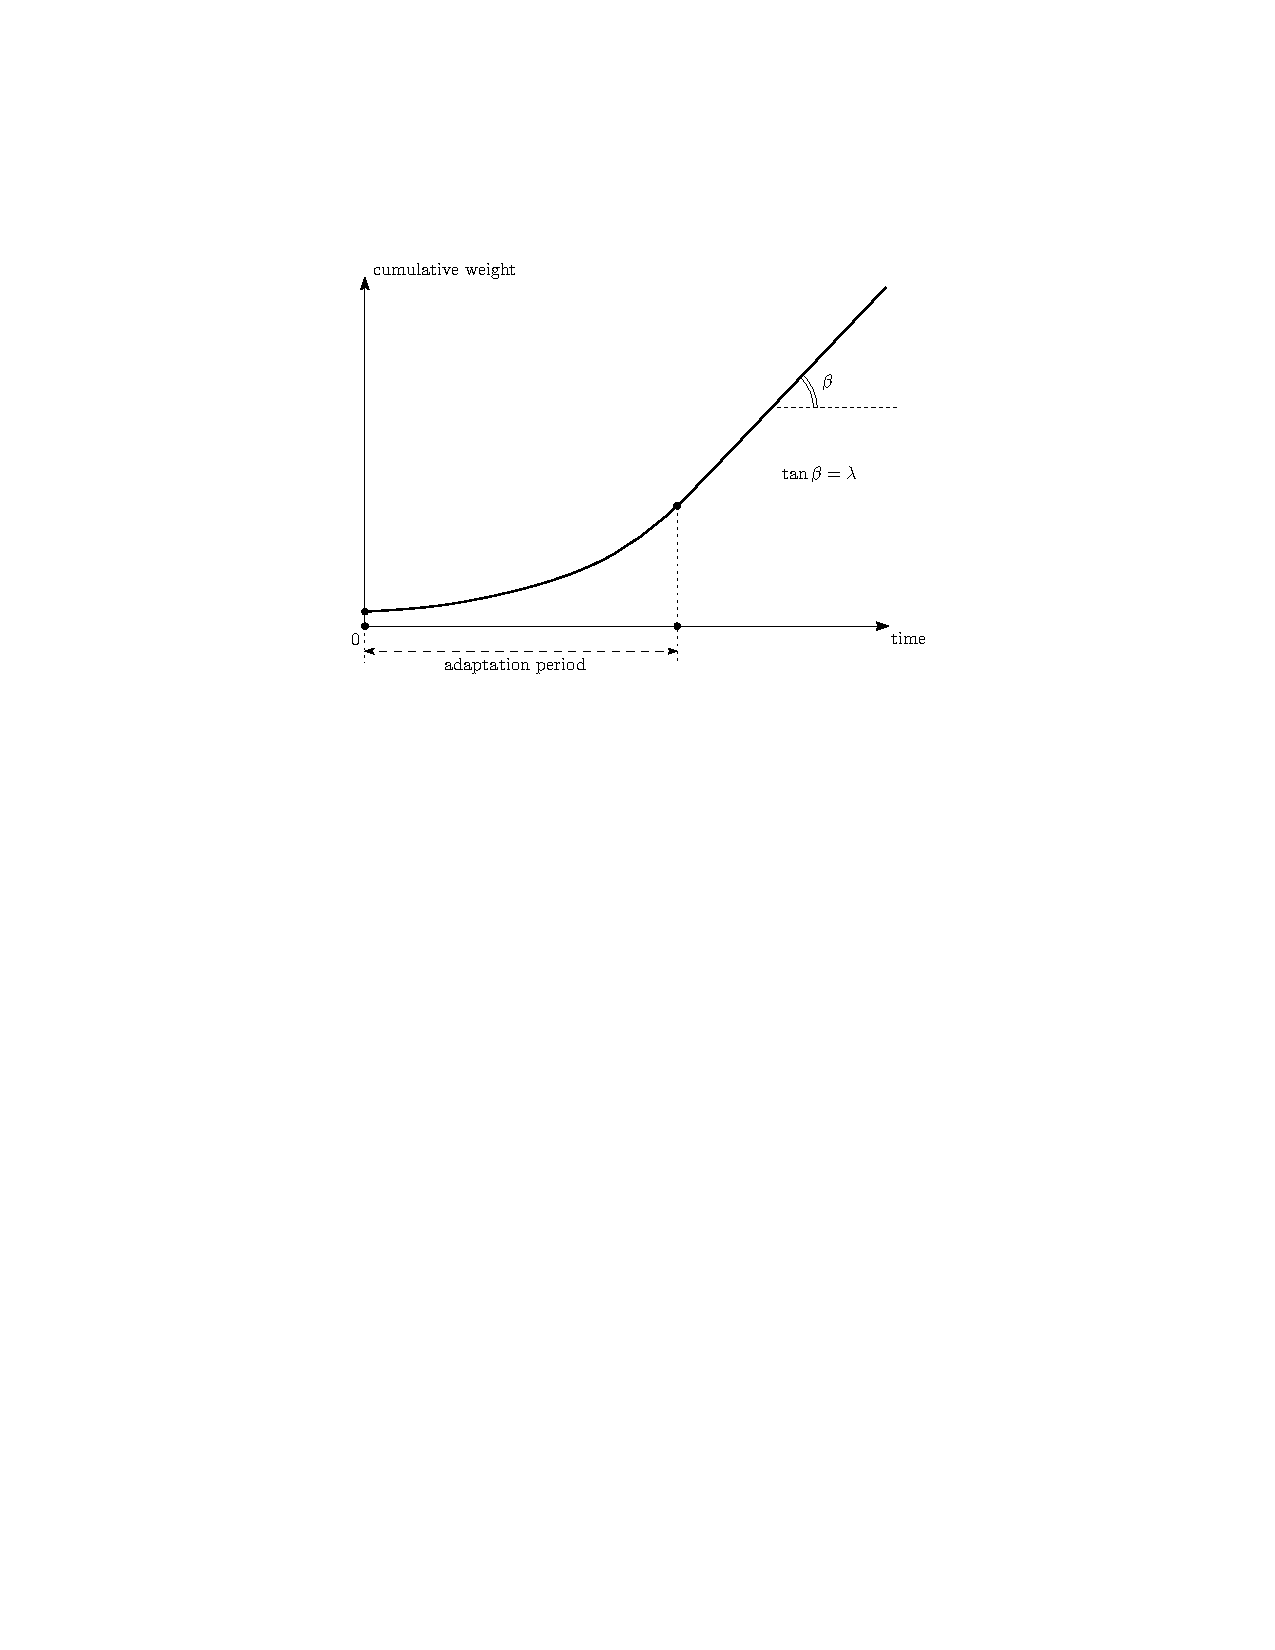
\includegraphics[width=8cm]{images/confirmation-confidence.pdf}
    \caption{Confirmation Confidence and Cumulative Weight Growth \cite{the-tangle}}
    \label{fig:confirmation-confidence}
\end{figure}

In Figure \ref{fig:confirmation-confidence-tangle}, transactions with confirmation confidence of more than 0.95 have a thick border. Almost any new honest transaction that is added to this tangle will confirm these transactions (except lazy nodes with lazy tip selection). In the shown example, transaction 9 confirms all the red transactions and is confirmed by the blue transactions. There are four tips in the shown simulation - 6, 10, 11 and 12. The confirmation confidence of transaction 9 is 0.94 due to the fact that transactions 10, 11 and 12 have more importance than 6.
Transaction 4 has confirmation confidence of 1 since all tips have a path to transaction 4 and therefore, there is no transaction in the network that does not confirm this transaction.

\begin{figure}[H]
    \centering
    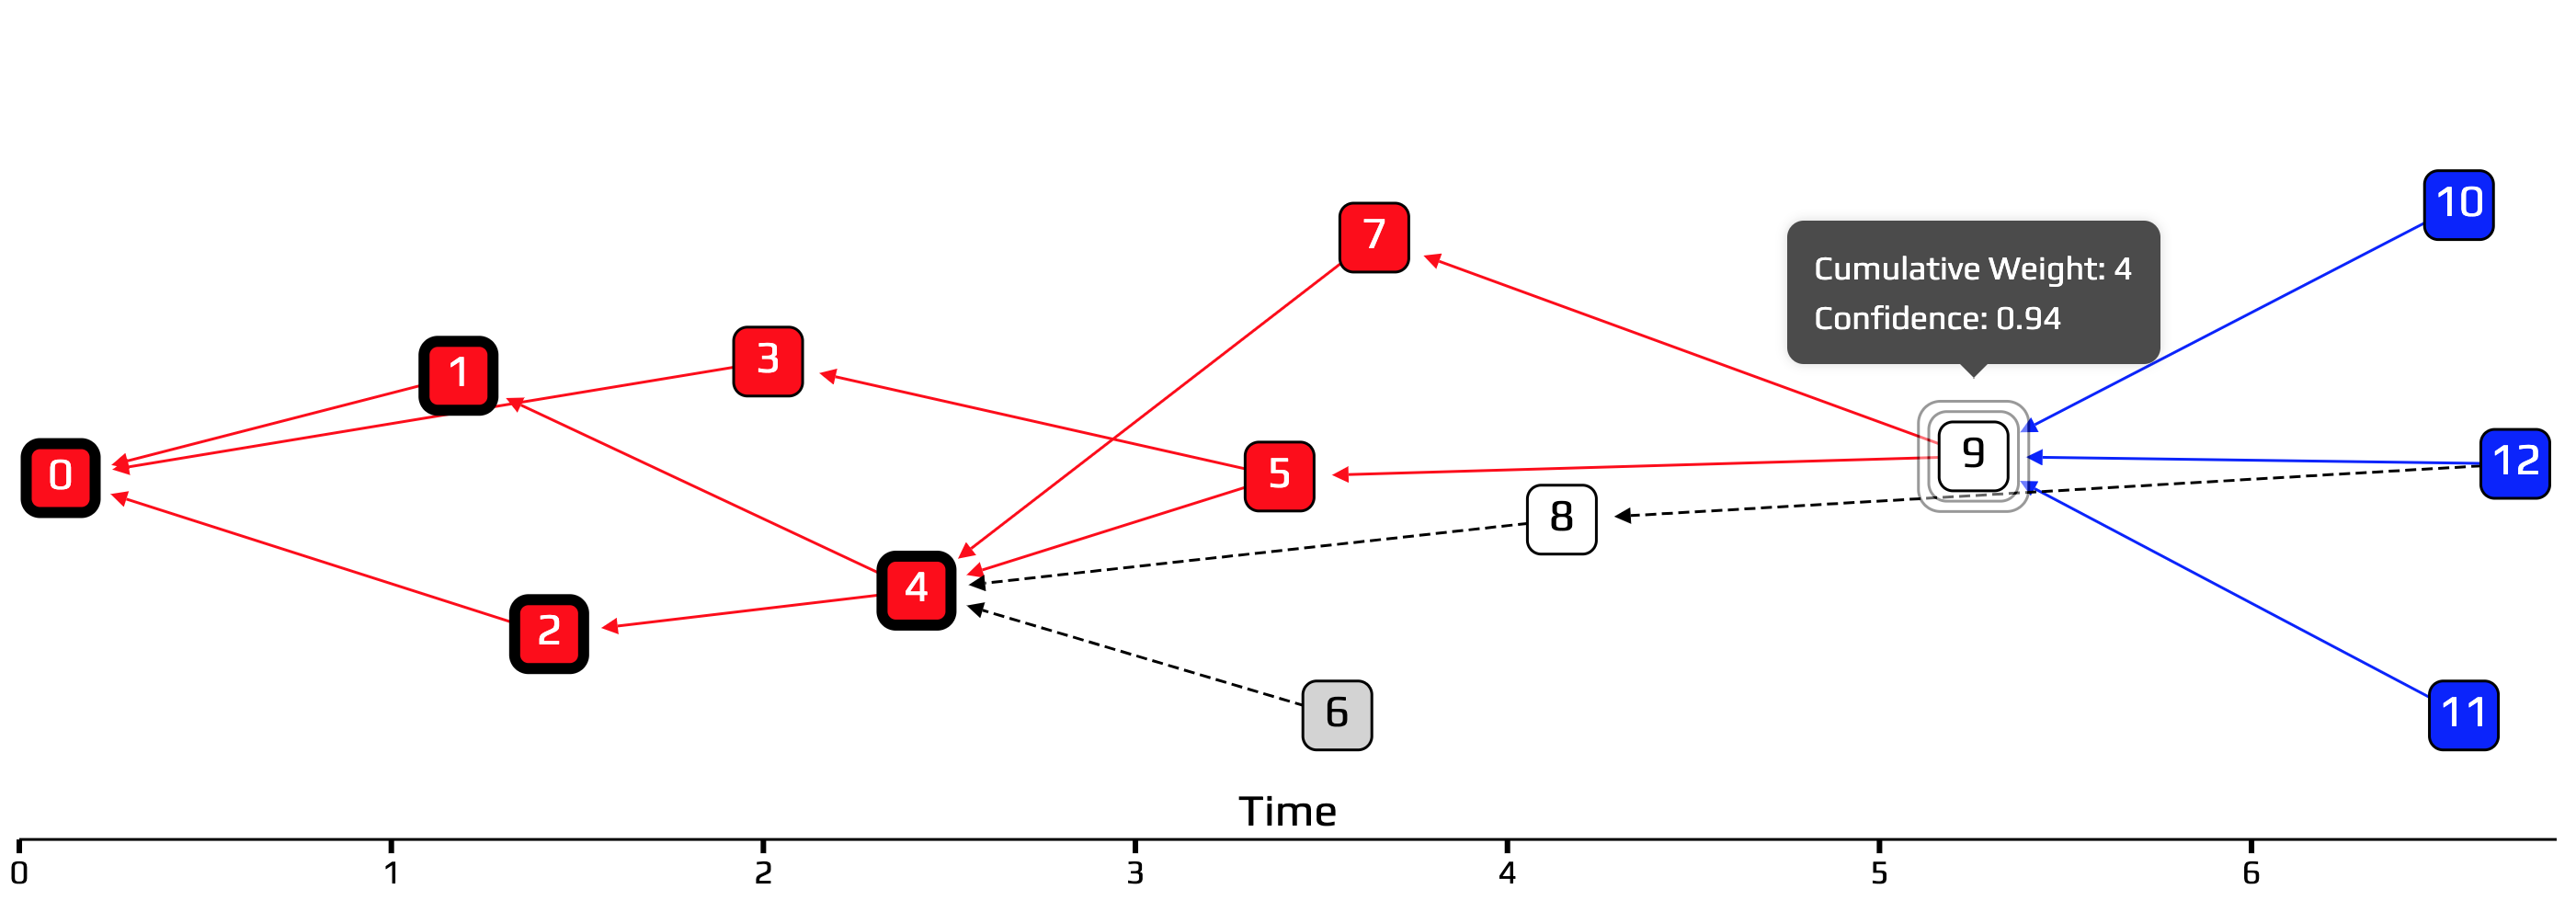
\includegraphics[width=1.0\textwidth]{images/confirmation-confidence-tangle.png}
    \caption{Graph Representation of the Confirmation Confidence}
    \label{fig:confirmation-confidence-tangle}
\end{figure}

\section{Coordinator}\label{coordinator}
In the early stages of the Tanlge, the network is susceptible to several attacks. Some of these attacks are discussed in Chapter \ref{attacks}. In summary, a user that controls a majority of the hashing power can double-spend coins. Unlike in Bitcoin where a miner competes with all other miners, in IOTA an attacker only competes with nodes that actively issue transactions! Thus, in times where not many transactions are issued, an attack becomes more feasible to execute.

In order to protect itself against such attacks, the IOTA foundation operates a special node called the Coordinator (Coo). This node has a checkpoint function. By issuing periodically zero-value transactions, the Coo creates milestones. Every transaction that is directly or indirectly confirmed by this milestone is considered as valid. The Coo is a central entity in the tangle and manifests a single point of failure. The Coo is not able to invalidate transactions from previous milestones. However, the node has several privileges compared to a regular node.

\begin{enumerate}
    \item The foundation can prioritize transactions.
    \item The Coo has the ability to censor transactions by continuously not approving certain transactions.
    \item If Coo is attacked and no longer works, the entire network halts.
\end{enumerate}

As such a central element is not desired in a decentralized system, the IOTA foundations investigates in possible solutions to this problem. These solution statements are explained in Section \ref{coo-less-tangle}.

\section{Qubic}\label{qubic}
The Qubic protocol addresses the integration of smart contracts (SC), oracles and outsourced computation within the IOTA network. The following terminology helps to understand the aim of the protocol.
\begin{description}
    \item[Qubic (QBC)] The protocol receives its name from quorum-based (distributed) computation.
    \item[quorum] A quorum is the minimum number of votes that a transaction/data must obtain, such that is is considered as valid. The introduction of quorum-based computation makes it more difficult for malicious nodes to falsify data as well as reduce noisy data from faulty sensors. 
    \item[qubic] Besides the protocols name, a qubic is also referred to a packaged quorum-based computation that occurs according to the Qubic protocol. One can think of a qubic as a data/computation request or task on the tangle. 
    \item[qubic owner] The qubic owner is the node that issues the request (qubic). For every qubic, a reward is defined. This reward is split among all nodes that enforce the quorum result. This promotes honest behavior, as a node is not rewarded when publishing a defective result.
    \item[(deliberative) assembly] A group of oracles forms an assembly where all of its members will process the same set of qubics. Each oracle will post its results for every qubic on the Tangle. The assembly will decide on the true value of the requested data. The threshold of the acceptance rate is usually set to $2/3$.
    \item[Abra] The IOTA foundation develops a functional programming language called Abra. It uses the trinary number system in order to save disk space and computational power.
\end{description}

The Qubic protocol is still in development and is not deployed on any testnet by date of writing this paper.

\subsection{Oracles}\label{oracles}
Oracles bring real-world data into the ledger. Difficulties that must be considered are the Sybil attack and the classroom attack, where oracles copy the result of other oracles without measuring the requested data.
\begin{description}
    \item[Sybil Attack] A single oracle could impersonate multiple oracles at the same time in order to receive a larger cut of the reward. Such a Sybil attack is most likely mitigated in the Qubic protocol by weighted voting. An oracle has a voting weight according to the resources it used to solve a crpytographic puzzle (PoW) or according to its stake in the network. These voting weights are set initially when a assembly is formed. However, it can be adjusted when new nodes join the assembly or when the majority of the assembly agrees on a new resource test phase. During this phase, the computational resources of each oracle are examined and the weights are updated accordingly.
    \item[Classroom attack] Results must be published in a commit-reveal schema, such that oracles cannot copy the results from others without verifying the data. 
\end{description}

\subsection{Outsourced computing}
Outsourced computing addresses the problem that not every IoT device is able to execute computationally complex tasks due to memory, computational power and energy availability limitations. As with oracle machines, outsourced computation is handled in a decentralized way, with the Qubic protocol ensuring that the results can be trusted to a high degree of certainty. The protocol allows anyone to request to run a computational task without permission. On the other hand, any node can become part of an assembly which will eventually be assigned to solve computational tasks.

\subsection{Smart Contracts}
Smart contracts facilitate, verify and enforce transactions on the underlying ledger technology without the need of a third party.

\subsection{Qubic in Action}
The following example illustrates how the three building blocks complete the Qubic protocol.

\begin{enumerate}
    \item The car insurance and the driver establish a \textbf{smart contract} that contains variable rates for different driving conditions. The cost depends on multiple factors. This data can be retrieved in a distributed manner by issuing qubics such as a temperature qubic, traffic jam qubic, etc.
    \item Autonomous cars could act as a group of \textbf{oracles} (assembly) when deciding on traffic congestion. If the quorum is set to $2/3$ and $2/3$ of the cars in a specific area register a high degree of traffic the tangle registers this information.
    \item Analyzing the data from the tangle might be \textbf{computationally} expensive. Thus, a new qubic is issued for analyzing the different factors from the tangle and is \textbf{outsourced} to a assembly that can compute this task efficiently.
    \item When the result of the analyzing qubic is received, the \textbf{smart contract} automatically pays the necessary amount for the car insurance according to the driving conditions.
\end{enumerate}





\chapter{Attack Scenarios}\label{attacks}

This section covers some of the possible attack scenarios and how the Tangle can still maintain consensus among honest users.

\section{Double Spend}
A double spend situation occurs when a user tries to exceed his account balance by issuing two or more conflicting transactions. Figure \ref{fig:double-spend} illustrates such a scenario. A box represents a transaction. The dashed box inside represents the current state in the graph but is not part of an actual transaction. In this simulation, Alice owns 15 IOTA but issues two outgoing transactions with 10 IOTA each. Bob cannot approve both of Alice's transactions as they result in a negative account balance.

\begin{figure}[H]
    \centering
    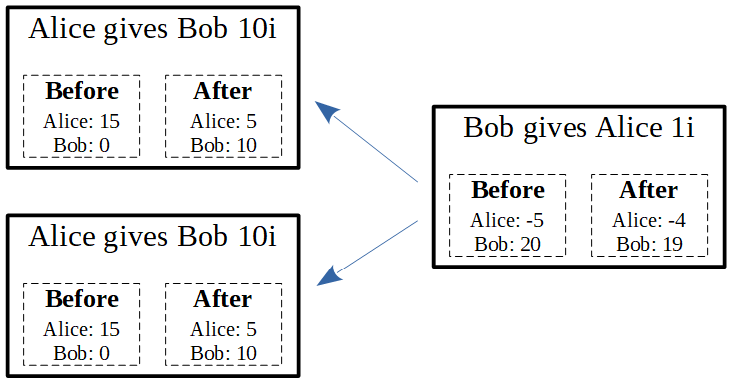
\includegraphics[width=8cm]{images/double-spend.png}
    \caption{Double Spend Attack \cite{the-tangle-part-5}}
    \label{fig:double-spend}
\end{figure}

The solution to this problematic situation is the weighted random walk discussed in Section \ref{tip-selection}. One of the two transactions will become heavier and the lighter one will be abandoned. This implies that a confirmed transaction cannot be considered as valid as soon as it has been approved for the first time. 

Confirmation confidence is introduced in Section \ref{transaction-validation} and provides a measurement of what percentage the network has directly or indirectly approved a transaction. 


\section{Large Weight Attack}
The large weight attack has the same intent as the double spend but actively tries to invalidate a transaction with high confirmation confidence. This can be achieved by a malicious user as follows.

\begin{enumerate}
    \item A transaction is created and broadcasted that is intended to revert.
    \item The malicious user waits until the receiver believes the transaction has a high enough confirmation rate. The merchant ships the product/service.
    \item The attacker uses its computational power and issues a double-spending transaction with a large weight followed by many more transactions. This transaction does not approve the first transaction and thus they compete with each other for finality.
    \item The bad actor hopes that the dishonest subtangle gains more cumulative weight than the honest subtangle.
\end{enumerate}

\begin{figure}[H]
    \centering
    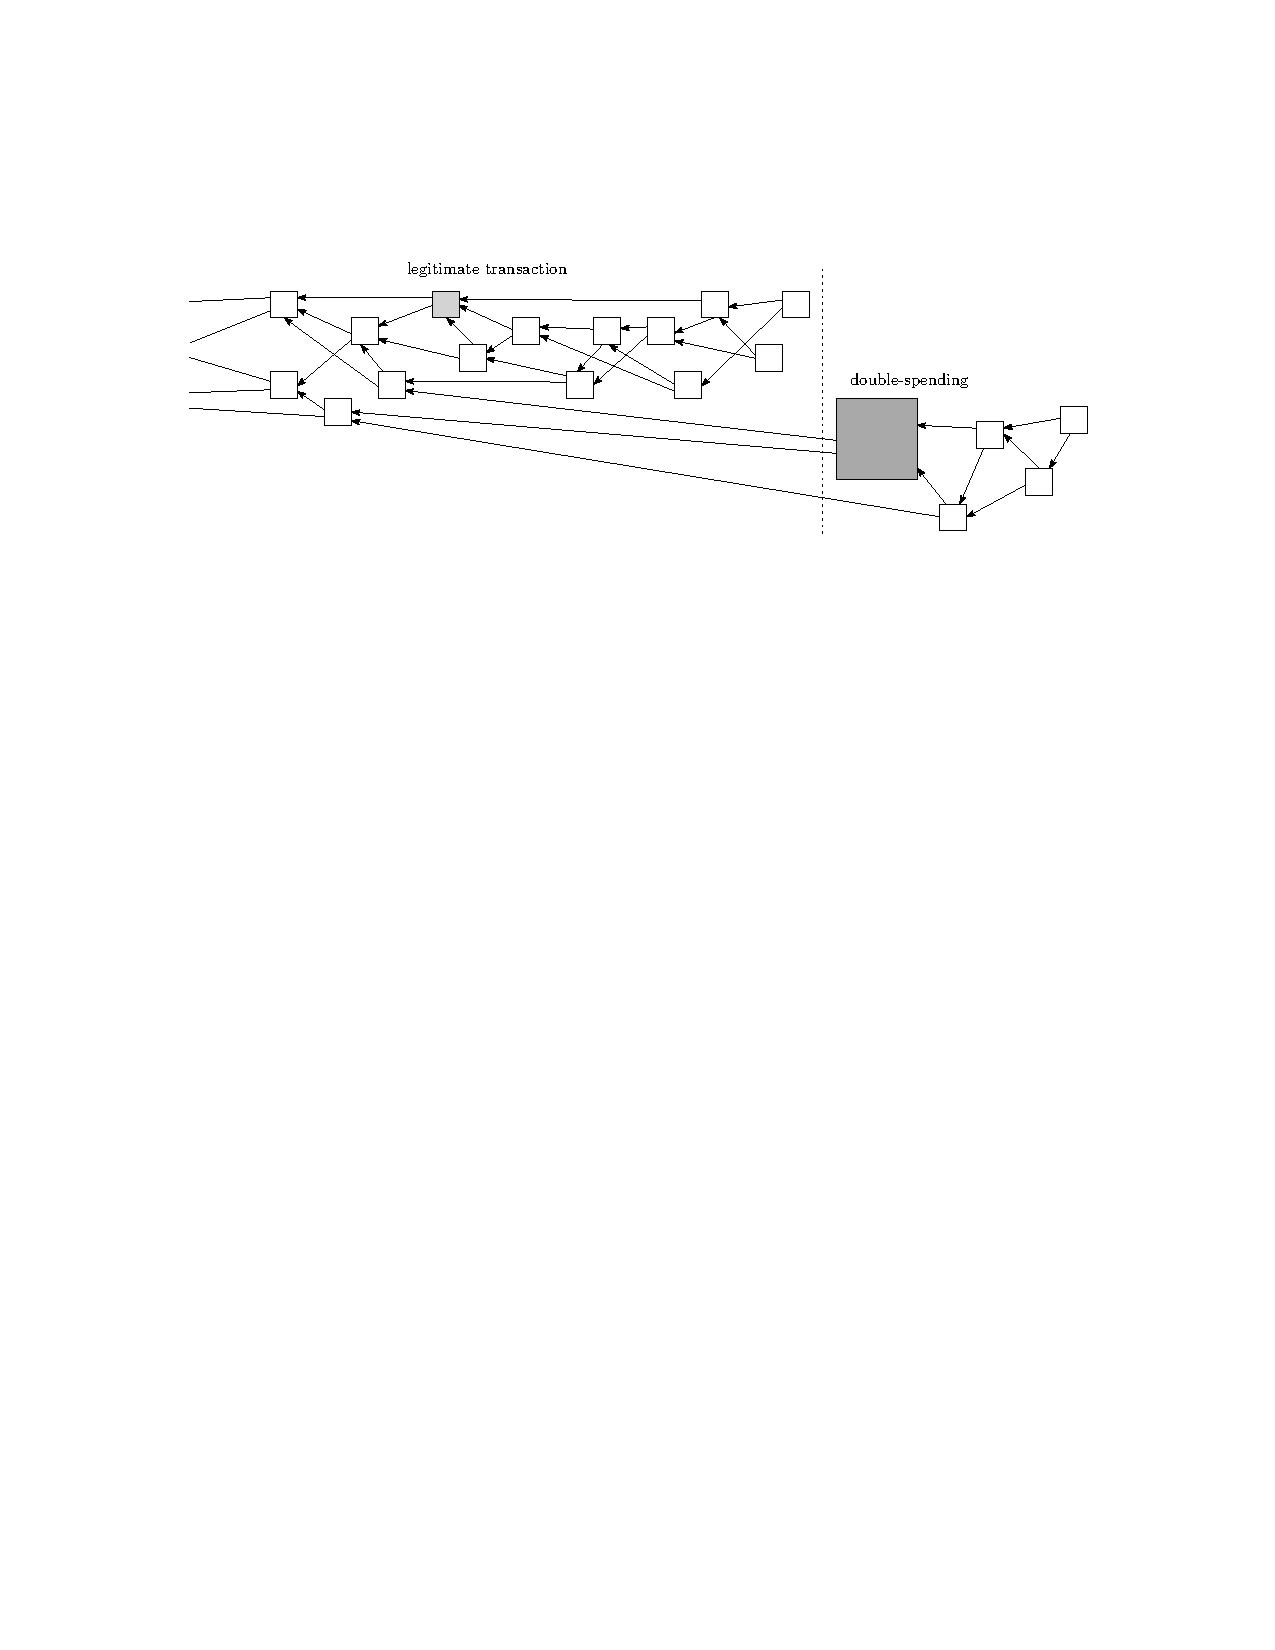
\includegraphics[width=12cm]{images/large-weight-attack.pdf}
    \caption{Large Weight Attack \cite{the-tangle}}
    \label{fig:large-weight-attack}
\end{figure}

This attack can only be carried out if the attacker has more computing power than all the nodes that actively issue new transactions. In a well-established network with many nodes issuing transactions, this is less of an issue. In the early stages, however, there are not enough transactions passing through the network in order to be safe from such an attack. Due to this reason, the IOTA foundation has put a coordinator in place which is discussed in more detail in Section ?.

\section{Parasite Chain Attack}
The parasite chain attack also tries to convince the network to abandon a previously confirmed transaction by biasing the tip selection algorithm. The attack works as follows:
\begin{enumerate}
    \item The attacker creates a transaction branching off from the main tangle (MT). He does not broadcast this transaction. This transaction is the red dot furthest to left in Figure \ref{fig:parasite-chain}.
    \item Instead, he keeps adding new transactions to this local chain called parasite chain (PC).
    \item He makes sure, that he references the MT within the PC.
    \item The malicious user creates a transaction on the MT which he hopes to get abandoned by the network when he publishes the parasite chain. This transaction is the red dot furthest to right.
    \item The user waits until the transaction on the MT is considered as validated. During this time he keeps building on the PC but can only reference transactions before the double-spend transaction on the MT.
    \item At this point, the bad actor broadcasts the parasite chain.
    \item Furthermore, he might try to artificially inflate the number of tips on the PC.
\end{enumerate}

The attacker's intention is that new transactions reference the parasite chain such that the MT will be orphaned. 
However, the tips on the parasite chain have a smaller amount of cumulative weight, assumed the attacker has less computational power than the rest of the network. 
Thus, in order to mitigate such an attack, it is important for the MCMC selection algorithm to be biased towards transactions with a high cumulative weight. The tradeoff for setting the bias is discussed in Section \ref{tip-selection}.

\begin{figure}[H]
    \centering
    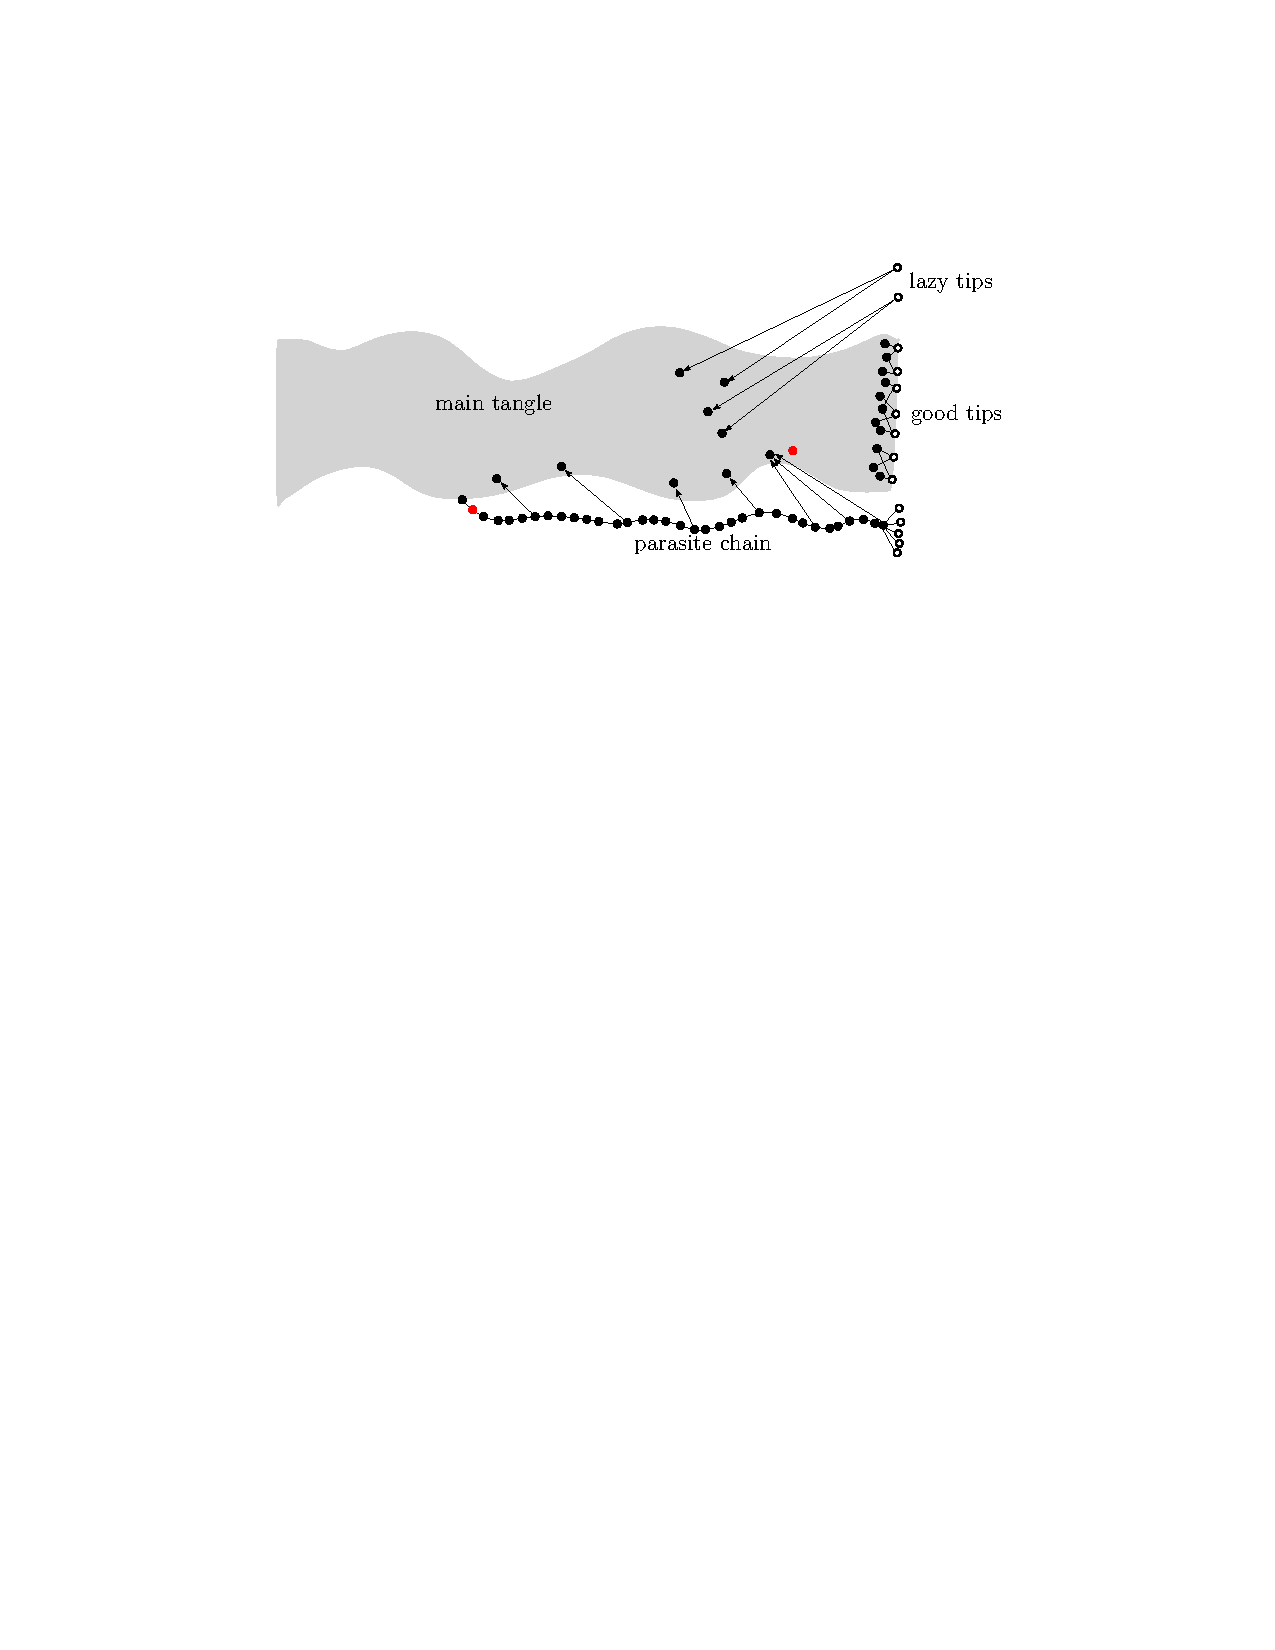
\includegraphics[width=12cm]{images/parasite-chain.pdf}
    \caption{Parasite Chain Attack \cite{the-tangle}}
    \label{fig:parasite-chain}
\end{figure}


\chapter{Research Topics}
Research topics that are actively ivestigated by the IOTA foundation are discussed within this Section.

\section{Coo-less Tangle}\label{coo-less-tangle}
The coordinator-free Tangle is developed by a dedicated research team of the IOTA foundation. There are three concepts proposed for a more decentralized network.
\begin{enumerate}
    \item \textbf{Node accountability} is a reputation system built into the protocol, similar to object reputation systems used in p2p file-sharing such as the Gnutella network \cite{object-reputation-system}. Such a protocol allows making judgments about the authenticity of incoming transactions. The reputation of a node is lowered whenever a node attempts to make a double-spend transaction or issues many re-attachments. Re-attachments are used in IOTA when a transaction is left behind on a branch that is likely to be abandoned.
    \item As mentioned in Section \ref{tip-selection}, the \textbf{tip selection algorithm} is one of the main difficulties in the network. Without the Coo, there are no milestones from which the MCMC random walk algorithm derives. Thus, a new heuristic algorithm is developed using backtracking from a recent tip until it reaches a transaction with a high cumulative weight.    
    \item The \textbf{Stars Concept} is an idea that works with well-known, public and trusted entities such as governments and corporations. These entities issue reference transactions which are similar to the milestones issued by the Coo.
\end{enumerate}

These approaches are implemented and tested on the so-called zero-value testnet (znet).


\section{Qubic}\label{qubic}
The Qubic protocol addresses the integration of smart contracts (SC), oracles and outsourced computation within the IOTA network. The following terminology helps to understand the aim of the protocol.
\begin{description}
    \item[Qubic (QBC)] The protocol receives its name from quorum-based (distributed) computation.
    \item[quorum] A quorum is the minimum number of votes that a transaction/data must obtain, such that is is considered as valid. The introduction of quorum-based computation makes it more difficult for malicious nodes to falsify data as well as reduce noisy data from faulty sensors. 
    \item[qubic] Besides the protocols name, a qubic is also referred to a packaged quorum-based computation that occurs according to the Qubic protocol. One can think of a qubic as a data/computation request or task on the tangle. 
    \item[qubic owner] The qubic owner is the node that issues the request (qubic). For every qubic, a reward is defined. This reward is split among all nodes that enforce the quorum result. This promotes honest behavior, as a node is not rewarded when publishing a defective result.
    \item[(deliberative) assembly] A group of oracles forms an assembly where all of its members will process the same set of qubics. Each oracle will post its results for every qubic on the Tangle. The assembly will decide on the true value of the requested data. The threshold of the acceptance rate is usually set to $2/3$.
    \item[Abra] The IOTA foundation develops a functional programming language called Abra. It uses the trinary number system in order to save disk space and computational power.
\end{description}

The Qubic protocol is still in development and is not deployed on any testnet by date of writing this paper.

\subsection{Oracles}\label{oracles}
Oracles bring real-world data into the ledger. Difficulties that must be considered are the Sybil attack and the classroom attack, where oracles copy the result of other oracles without measuring the requested data.
\begin{description}
    \item[Sybil Attack] A single oracle could impersonate multiple oracles at the same time in order to receive a larger cut of the reward. Such a Sybil attack is most likely mitigated in the Qubic protocol by weighted voting. An oracle has a voting weight according to the resources it used to solve a crpytographic puzzle (PoW) or according to its stake in the network. These voting weights are set initially when a assembly is formed. However, it can be adjusted when new nodes join the assembly or when the majority of the assembly agrees on a new resource test phase. During this phase, the computational resources of each oracle are examined and the weights are updated accordingly.
    \item[Classroom attack] Results must be published in a commit-reveal schema, such that oracles cannot copy the results from others without verifying the data. 
\end{description}

\subsection{Outsourced computing}
Outsourced computing addresses the problem that not every IoT device is able to execute computationally complex tasks due to memory, computational power and energy availability limitations. As with oracle machines, outsourced computation is handled in a decentralized way, with the Qubic protocol ensuring that the results can be trusted to a high degree of certainty. The protocol allows anyone to request to run a computational task without permission. On the other hand, any node can become part of an assembly which will eventually be assigned to solve computational tasks.

\subsection{Smart Contracts}
Smart contracts facilitate, verify and enforce transactions on the underlying ledger technology without the need of a third party.

\subsection{Qubic in Action}
The following example illustrates how the three building blocks complete the Qubic protocol.

\begin{enumerate}
    \item The car insurance and the driver establish a \textbf{smart contract} that contains variable rates for different driving conditions. The cost depends on multiple factors. This data can be retrieved in a distributed manner by issuing qubics such as a temperature qubic, traffic jam qubic, etc.
    \item Autonomous cars could act as a group of \textbf{oracles} (assembly) when deciding on traffic congestion. If the quorum is set to $2/3$ and $2/3$ of the cars in a specific area register a high degree of traffic the tangle registers this information.
    \item Analyzing the data from the tangle might be \textbf{computationally} expensive. Thus, a new qubic is issued for analyzing the different factors from the tangle and is \textbf{outsourced} to a assembly that can compute this task efficiently.
    \item When the result of the analyzing qubic is received, the \textbf{smart contract} automatically pays the necessary amount for the car insurance according to the driving conditions.
\end{enumerate}


\section{Economic Clustering}\label{economic-clustering}

Economic clustering is a theoretical approach for more scalability. It is inspired by global real-world economies. The global economy is divided up into regional economies. These local economies coexist but do not influence each other. 

When this concept of global economies is applied to IOTA, each of these local economies represents a cluster. Clusters run their own tangle. Clusters are not compatible and one can only transact within a cluster. Thus, there is a need for inter-cluster exchanges, which are users or institutions that have funds in multiple clusters. 

\chapter{Evaluation}


\chapter{Summary and Conclusions}

The fact that every node in the network that wants to participate has to confirm other transactions, make the network more decentralized than most current blockchain implementations. The chosen signature scheme for quantum resistance makes sense with the emerging technological advancements in this area. 

However, the fact that the IOTA protocol uses PoW as an anti-spam mechanism makes the network not practical for battery-powered IoT devices with low performance CPUs. 

There are no solutions for the storage problem that do not affect the security of the network. Using the tangle for decentralized storage has problematic incentive structures as it is almost free to store but costs to read data. Furthermore, the tangle is prone to a single-point of failure as the coordinator is operated by a single party.

Due to these reasons, the current implementation of the protocol has too many flaws to build a real-world application which has to rely on the tangle.


\begin{thebibliography}{99}
\addcontentsline{toc}{chapter}{Bibliography}

\bibitem{label} Autoren: Titel, Verlag, \url{http://...}, Datum.
\bibitem{the-tangle} Serguei Popov: The Tangle - Version 1.4.3, \url{https://assets.ctfassets.net/r1dr6vzfxhev/2t4uxvsIqk0EUau6g2sw0g/45eae33637ca92f85dd9f4a3a218e1ec/iota1_4_3.pdf}, 30th of April 2018, accessed 20th of Mai 2019..
\bibitem{the-tangle-part-1} Alon Gal: The Tangle: an illustrated introduction, \url{https://blog.iota.org/the-tangle-an-illustrated-introduction-f359b8b2ec80}, 31st of January 2018, accessed 20th of Mai 2019.
\bibitem{the-tangle-part-2} Alon Gal: The Tangle: an illustrated introduction - Part 2: transaction rates, latency, and random walks, \url{https://blog.iota.org/the-tangle-an-illustrated-introduction-f359b8b2ec80}, 7th of February 2018, accessed 20th of Mai 2019.
\bibitem{the-tangle-part-3} Alon Gal: The Tangle: an illustrated introduction - Part 3: Cumulative weights and weighted random walks, \url{https://blog.iota.org/the-tangle-an-illustrated-introduction-f359b8b2ec80}, 14th of February 2018, accessed 20th of Mai 2019.
\bibitem{the-tangle-part-4} Alon Gal: The Tangle: an illustrated introduction - Part 4: Approvers, balances, and double-spends, \url{https://blog.iota.org/the-tangle-an-illustrated-introduction-f359b8b2ec80}, 21st of February 2018, accessed 20th of Mai 2019.
\bibitem{the-tangle-part-5} Alon Gal: The Tangle: an illustrated introduction - Part 5: Consensus, confirmation confidence, and the coordinator, \url{https://blog.iota.org/the-tangle-an-illustrated-introduction-f359b8b2ec80}, 28th of February 2018, accessed 20th of Mai 2019.
\bibitem{mcmc} Ben Shaver: A Zero-Math Introduction to Markov Chain Monte Carlo Methods, \url{https://towardsdatascience.com/a-zero-math-introduction-to-markov-chain-monte-carlo-methods-dcba889e0c50}, 22nd of Dezember 2017, accessed 20th of Mai 2019.
\bibitem{poisson-process} Will Koehrsen: The Poisson Distribution and Poisson Process Explained, \url{https://towardsdatascience.com/the-poisson-distribution-and-poisson-process-explained-4e2cb17d459}, 21st of January 2019, accessed 20th of Mai 2019.
\bibitem{parasite-chain} Bartosz Kusmierz: Attack analysis - the simple parasite chain \url{https://blog.iota.org/attack-analysis-the-simple-parasite-chain-42a34bfeaf23}, 10th of October 2019, accessed 20th of Mai 2019.


\end{thebibliography}



\chapter*{Abbreviations}
\addcontentsline{toc}{chapter}{Abbreviations}
\markboth{ABBREVIATONS}{}

\abr{MBM}{Master Basis Module}
\abr{SC}{Smart Contract}
\abr{MCMC}{Markov Chain Monte Carlo}
\abr{DAG}{Directed Acyclic Graph}
\abr{IF}{IOTA Foundation}
\abr{IoT}{Internet of Things}
\abr{UTXO}{Unspent Transaction Output}
\abr{MIOTA}{Mega IOTA (Equivalent to 1 Million IOTA)}
\abr{MT}{Main Tangle}
\abr{PC}{Parasite Chain}
\abr{TPS}{Transactions Per Second}
\abr{Coo}{short for Coordicile}
\abr{IRI}{IOTA Reference Implementation}
\abr{CLIRI}{Cooridinator-Less IOTA Reference Implementation}
\chapter*{Glossary}
\addcontentsline{toc}{chapter}{Glossary}
\markboth{GLOSSARY}{}


\begin{description}
  \item[IOTA] IOTA is the name of the smallest unit in the crypto currency created by the IOTA Foundation. Most exchanges use MIOTA which is equivalent to 1 Million IOTA.
  \item[Lazy Tips] A node in the network which does not confirm the most recent transactions creates lazy tips.
  \item[Tangle] The underlying graph data sturcture in IOTA is called Tangle.
\end{description}


\addcontentsline{toc}{chapter}{List of Figures}
\listoffigures
\addcontentsline{toc}{chapter}{List of Tables}
\listoftables

\appendix

\chapter{Installation Guidelines}

\chapter{Contents of the CD}


\end{document}
